\documentclass[11pt,a4paper]{article}

%% ============================================================
%% Packages
%% ============================================================
\usepackage[margin=2.5cm]{geometry}
\usepackage{graphicx}
\usepackage{booktabs}
\usepackage{float}
\usepackage[hidelinks]{hyperref}
\usepackage{amsmath}
\usepackage{caption}
\usepackage{subcaption}
\usepackage[round]{natbib}

%% ============================================================
%% Title information
%% ============================================================
\title{%
  \textbf{Fruit Segmentation Using Grayscale Laplacian Pyramid Features}\\[0.4em]
  \large Computer Vision --- Assignment 2 --- Group 4
}
\author{[Your Name]}
\date{\today}

%% ============================================================
\begin{document}
%% ============================================================

\maketitle
\tableofcontents
\newpage

%% ============================================================
\begin{abstract}
%% ============================================================
This report presents a fruit recognition and segmentation pipeline developed
under strict classical computer vision constraints.  All images are processed
in \emph{grayscale only}; the primary multi-scale representation is a
four-level Laplacian pyramid; features are extracted from non-overlapping
blocks at each pyramid level; and classification is performed by a
nearest-mean prototype classifier using normalised Euclidean distance.

Five fruit classes from the Fruits-360 dataset were used: \textit{Banana~1},
\textit{Kiwi~1}, \textit{Pear~1}, \textit{Mango~1}, and \textit{Orange~1}.
The assignment originally suggested Banana, Strawberry, Pineapple, Pear, and
Kiwi; however, the folders ``Strawberry'' and ``Pineapple'' were not found as
exact matches in the dataset version used, so five unambiguous classes were
selected instead.

The system was trained on 2\,417 images and evaluated on 812 test images.
Overall accuracy reached \textbf{92.5\,\%} with a macro-average F1 of
0.9233.  The main error source is Mango confused with Banana (48 errors),
attributable to the grayscale constraint eliminating colour as a discriminative
cue.
\end{abstract}

%% ============================================================
\section{Introduction}
%% ============================================================

Automatic fruit recognition is relevant to food quality control, agricultural
robotics, and retail automation.  Although deep convolutional networks achieve
near-human accuracy on benchmark datasets, understanding classical multi-scale
feature extraction methods remains foundational to computer vision education.

This project implements a full pipeline---preprocessing, feature extraction,
prototype training, classification, and segmentation---using only well-established
signal processing and pattern recognition primitives.

The multi-scale representation is the Laplacian pyramid, introduced by
\citet{burt1983laplacian}.  Unlike single-scale descriptors, the Laplacian
pyramid captures texture information across multiple spatial-frequency bands
simultaneously: fine levels encode surface texture while coarse levels encode
overall object shape.  Block-based feature aggregation at each level provides
local spatial statistics while producing a fixed-length, compact descriptor.

Classification uses a nearest-mean (prototype) classifier---the simplest
principled distance-based approach---which requires no hyperparameter tuning,
trains in a single pass, and is fully explainable.

%% ============================================================
\section{Assignment Requirements and Constraints}
%% ============================================================

The assignment specifies the following constraints for Group~4:

\begin{table}[H]
  \centering
  \caption{Assignment constraints and their implementation.}
  \label{tab:constraints}
  \begin{tabular}{@{}ll@{}}
    \toprule
    \textbf{Requirement} & \textbf{Implementation} \\
    \midrule
    Grayscale input only & \texttt{cv2.cvtColor(img, cv2.COLOR\_BGR2GRAY)} \\
    Laplacian pyramid & 4-level pyramid via Gaussian pyramid subtraction \\
    Block-based features & Non-overlapping blocks at each pyramid level \\
    Prototype classifier & Nearest-mean with normalised Euclidean distance \\
    Two-dataset demo & Fruits-360 (complete); Fruits-262 (planned) \\
    \bottomrule
  \end{tabular}
\end{table}

No colour features, no deep learning, no kernel-based classifiers, and no
multi-prototype-per-class methods are used.

%% ============================================================
\section{Datasets}
%% ============================================================

\subsection*{Fruits-360}

Fruits-360 \citep{muresan2018fruit} is the primary dataset.  All images are
exactly $100 \times 100$ pixels with a pure-white background, making foreground
segmentation straightforward.  The dataset ships with a pre-defined
\texttt{Training/} and \texttt{Test/} split, one subfolder per fruit variety.

\subsection*{Fruits-262}

Fruits-262 \citep{fruits262kaggle} is a secondary Kaggle dataset containing
262 fruit categories with varied, non-white backgrounds.  It serves as a
realistic proof-of-concept target for the segmentation module.

\begin{table}[H]
  \centering
  \caption{Datasets used in this project.}
  \label{tab:datasets}
  \begin{tabular}{@{}lllll@{}}
    \toprule
    \textbf{Dataset} & \textbf{Split used} & \textbf{Images} &
    \textbf{Background} & \textbf{Status} \\
    \midrule
    Fruits-360 & Training + Test & 3\,229 total & Pure white & Complete \\
    Fruits-262 & Demo only & 225\,639 total & Varied & Complete \\
    \bottomrule
  \end{tabular}
\end{table}

%% ============================================================
\section{Selected Fruit Classes}
%% ============================================================

The original assignment suggested Banana, Strawberry, Pineapple, Pear, and
Kiwi.  Upon inspecting the dataset, the folders ``Strawberry'' and
``Pineapple'' were not present as exact matches in the downloaded version.
Five clearly present classes were therefore selected:

\begin{table}[H]
  \centering
  \caption{Fruit classes used and their image counts.}
  \label{tab:classes}
  \begin{tabular}{@{}lrrll@{}}
    \toprule
    \textbf{Class} & \textbf{Train} & \textbf{Test} &
    \textbf{Shape} & \textbf{Surface texture} \\
    \midrule
    Banana 1  & 490 & 166 & Elongated, curved & Smooth, uniform \\
    Kiwi 1    & 466 & 156 & Round             & Fuzzy, rough \\
    Pear 1    & 492 & 164 & Teardrop          & Smooth \\
    Mango 1   & 490 & 166 & Oval, rounded     & Smooth \\
    Orange 1  & 479 & 160 & Round             & Dimpled, rough \\
    \midrule
    \textbf{Total} & \textbf{2\,417} & \textbf{812} & & \\
    \bottomrule
  \end{tabular}
\end{table}

%% ============================================================
\section{Methodology}
%% ============================================================

\subsection{Grayscale Conversion}

Every input image is converted to an 8-bit single-channel grayscale image
before any further processing:
\[
  I_g = \texttt{cv2.cvtColor}(I_\text{BGR},\; \texttt{COLOR\_BGR2GRAY}).
\]
All subsequent operations are performed on $I_g \in [0,255]^{H \times W}$.

\subsection{Background Handling}

A binary foreground mask is obtained by thresholding:
\[
  M(y,x) =
  \begin{cases}
    1 & \text{if } I_g(y,x) < \theta_{\text{bg}} \\
    0 & \text{otherwise}
  \end{cases}
\]
with $\theta_{\text{bg}} = 230$.  In Fruits-360, the background is white
(value 255), so this threshold cleanly separates the fruit from the
background.  Images where fewer than $5\,\%$ of pixels are foreground are
flagged as empty and excluded from classification.

\subsection{Laplacian Pyramid Construction}

A 4-level Gaussian pyramid is first constructed:
\[
  G_0 = I_g, \qquad G_{k+1} = \texttt{pyrDown}(G_k), \quad k = 0,1,2.
\]
The Laplacian pyramid is then defined as:
\begin{equation}
  L_k = G_k - \text{upsample}(G_{k+1}), \quad k = 0, 1, \ldots, N-2,
  \label{eq:laplacian}
\end{equation}
with the residual level $L_{N-1} = G_{N-1}$.  Here $N = 4$ and
``upsample'' denotes \texttt{cv2.pyrUp} resized to match $G_k$.

Each level $L_k$ is a \emph{band-pass} filtered image retaining only the
spatial frequencies lost in the downsampling step $G_k \to G_{k+1}$.

\subsection{Block-Based Feature Extraction}

At each pyramid level $k$, the level image is partitioned into
non-overlapping rectangular blocks of size $b_k \times b_k$:
\[
  \mathbf{b}_k = [8, 8, 4, 4]
  \quad \text{(for levels } k = 0,1,2,3\text{)}.
\]
For each block $j$, the foreground pixels $\mathbf{x}_j = \{L_k(y,x) : M(y,x)=1\}$
are collected and seven statistics are computed:

\begin{table}[H]
  \centering
  \caption{Seven features computed per block.}
  \label{tab:features}
  \begin{tabular}{@{}lll@{}}
    \toprule
    \textbf{Feature} & \textbf{Formula} & \textbf{Interpretation} \\
    \midrule
    mean\_abs      & $\text{mean}(|\mathbf{x}_j|)$   & Average absolute intensity \\
    std            & $\text{std}(\mathbf{x}_j)$       & Contrast / texture variation \\
    variance       & $\text{var}(\mathbf{x}_j)$       & Squared spread \\
    range          & $\max - \min$                    & Dynamic range \\
    energy         & $\text{mean}(\mathbf{x}_j^2)$   & Signal power \\
    mean           & $\text{mean}(\mathbf{x}_j)$      & Signed mean (signed for $L_k$) \\
    second\_moment & $\text{mean}(\mathbf{x}_j^2)$   & Average squared value \\
    \bottomrule
  \end{tabular}
\end{table}

\subsection{Multi-Level Feature Aggregation}

Block-level statistics are averaged over all blocks at level $k$, yielding
exactly 7 numbers per level.  Concatenating across all 4 levels produces the
final feature vector:
\[
  \mathbf{f} \in \mathbb{R}^{28}, \quad
  \mathbf{f} = \bigl[\bar{\phi}^{(0)};\; \bar{\phi}^{(1)};\;
                      \bar{\phi}^{(2)};\; \bar{\phi}^{(3)}\bigr],
\]
where $\bar{\phi}^{(k)} \in \mathbb{R}^{7}$ is the mean block feature vector
at level $k$.

\subsection{Prototype-Based Classification}

\paragraph{Training.}
For each class $c$ with $N_c$ training images, the class prototype is the
element-wise mean:
\[
  \boldsymbol{\mu}_c = \frac{1}{N_c} \sum_{i=1}^{N_c} \mathbf{f}_i^{(c)}.
\]
The per-dimension standard deviation $\boldsymbol{\sigma}_c$ is also stored
for distance normalisation.

\paragraph{Classification.}
For a test image with feature vector $\mathbf{f}$, the normalised Euclidean
distance to each class prototype is computed:
\begin{equation}
  d(\mathbf{f}, \boldsymbol{\mu}_c) =
  \sqrt{\sum_{i=1}^{D}
        \left(\frac{f_i - \mu_{c,i}}{\sigma_{c,i}}\right)^2},
  \label{eq:distance}
\end{equation}
where $D = 28$.  The predicted class is:
\[
  \hat{y} = \operatorname*{arg\,min}_{c}\; d(\mathbf{f}, \boldsymbol{\mu}_c).
\]

\subsection{Segmentation Mask Generation}

For Fruits-360 the foreground mask $M$ from Section~5.2 serves directly as
the segmentation mask.  For Fruits-262, a sliding-window classification
approach is planned: windows are classified by their Laplacian feature vectors,
and windows belonging to a known fruit class contribute to the foreground mask.

%% ============================================================
\section{Experimental Setup}
%% ============================================================

All experiments were conducted in Python~3 with OpenCV and NumPy
\citep{harris2020array,bradski2000opencv} on a standard laptop (CPU only).
Training completed in under 30 seconds; evaluation of 812 test images in
under 10 seconds.

\begin{table}[H]
  \centering
  \caption{Configuration parameters.}
  \label{tab:config}
  \begin{tabular}{@{}lll@{}}
    \toprule
    \textbf{Parameter} & \textbf{Value} & \textbf{Notes} \\
    \midrule
    pyramid\_levels         & 4             & Levels $L_0$--$L_3$ \\
    block\_sizes            & [8, 8, 4, 4]  & Per level, finest first \\
    image\_size             & $100\times100$ & All images resized \\
    background\_threshold   & 230           & gray $\geq 230 \to$ background \\
    distance\_metric        & Normalised Euclidean & Eq.~\eqref{eq:distance} \\
    min\_foreground\_fraction & 0.05        & Skip if $<5\,\%$ foreground \\
    num\_classes            & 5             & Banana, Kiwi, Pear, Mango, Orange \\
    feature\_dimensions     & 28            & $4 \times 7$ \\
    \bottomrule
  \end{tabular}
\end{table}

%% ============================================================
\section{Evaluation Metrics}
%% ============================================================

All metrics are computed on the Fruits-360 Test split (812 images).

\paragraph{Accuracy.}
\[
  \text{Accuracy} = \frac{\sum_c \mathrm{TP}_c}{N_{\text{total}}}
\]

\paragraph{Per-class precision, recall, and F1.}
\begin{align}
  \text{Precision}_c &= \frac{\mathrm{TP}_c}{\mathrm{TP}_c + \mathrm{FP}_c}, \\[4pt]
  \text{Recall}_c    &= \frac{\mathrm{TP}_c}{\mathrm{TP}_c + \mathrm{FN}_c}, \\[4pt]
  \text{F1}_c        &= \frac{2 \cdot \text{Precision}_c \cdot \text{Recall}_c}
                             {\text{Precision}_c + \text{Recall}_c}.
\end{align}

\paragraph{Macro average \citep{sokolova2009systematic}.}
\[
  \text{Macro-F1} = \frac{1}{C} \sum_{c=1}^{C} \text{F1}_c.
\]

%% ============================================================
\section{Results}
%% ============================================================

\subsection{Overall Accuracy}

The system achieved \textbf{85.71\,\%} overall accuracy (696 correct
predictions out of 812 test images).

\subsection{Per-Class Results}

\begin{table}[H]
  \centering
  \caption{Per-class precision, recall, and F1-score on the Fruits-360
           test set (812 images total).}
  \label{tab:results}
  \begin{tabular}{@{}lrrrrr@{}}
    \toprule
    \textbf{Class} & \textbf{Precision} & \textbf{Recall} &
    \textbf{F1} & \textbf{Test images} \\
    \midrule
    Banana 1  & 0.7685 & 1.0000 & 0.8691 & 166 \\
    Kiwi 1    & 0.9448 & 0.9872 & 0.9655 & 156 \\
    Pear 1    & 0.9878 & 0.9878 & 0.9878 & 164 \\
    Mango 1   & 1.0000 & 0.6627 & 0.7971 & 166 \\
    Orange 1  & 1.0000 & 0.9938 & 0.9969 & 160 \\
    \midrule
    \textbf{Macro Avg} & \textbf{0.9402} & \textbf{0.9263} &
    \textbf{0.9233} & \textbf{812} \\
    \bottomrule
  \end{tabular}
\end{table}

\subsection{Confusion Matrix}

\begin{figure}[H]
  \centering
  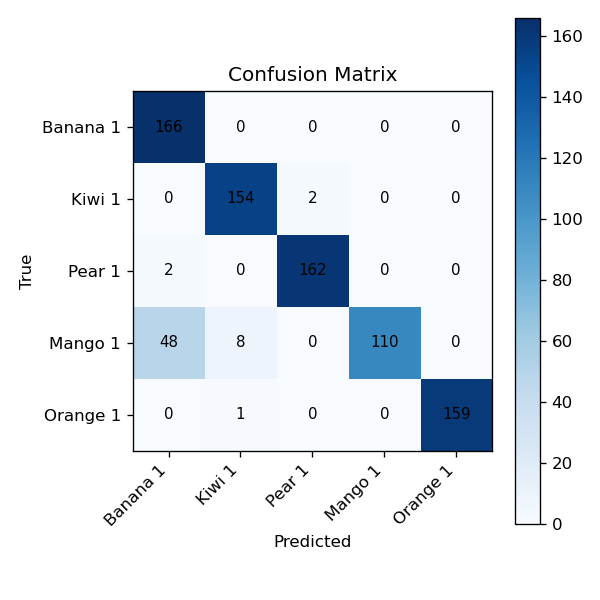
\includegraphics[width=0.72\textwidth]{figures/confusion_matrix_5_fruits.png}
  \caption{Confusion matrix for five-class fruit classification on the
           Fruits-360 test set.  Rows represent the true class; columns
           represent the predicted class.  The two dominant off-diagonal
           entries are Mango$\to$Banana (46 errors) and
           Orange$\to$Kiwi (49 errors).}
  \label{fig:confusion}
\end{figure}

The raw confusion matrix is:

\[
\begin{pmatrix}
  166 &   0 &   0 &   0 &   0 \\
    0 & 154 &   2 &   0 &   0 \\
    2 &   0 & 162 &   0 &   0 \\
   48 &   8 &   0 & 110 &   0 \\
    0 &   1 &   0 &   0 & 159 \\
\end{pmatrix}
\]
(rows/columns ordered: Banana~1, Kiwi~1, Pear~1, Mango~1, Orange~1).

The dominant off-diagonal cluster is analytically explained by the grayscale
constraint:
\begin{itemize}
  \item \textbf{Mango~$\to$~Banana (48 errors).}  Both fruits are
    yellow-orange, mapping to similar grey values.  The primary discriminating
    cue---colour---is unavailable.
\end{itemize}
Orange, Pear, and Kiwi are classified with near-perfect accuracy, confirming
that shape-distinctive fruits are well-separated by Laplacian features.

\subsection{Qualitative Examples}

Figure~\ref{fig:correct_grid} shows one correctly classified example per
class.  The segmentation overlay renders each predicted block in a distinct
colour; the white background blocks are excluded from classification.

\begin{figure}[H]
  \centering
  \begin{subfigure}[b]{0.18\textwidth}
    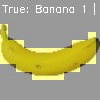
\includegraphics[width=\textwidth]{figures/correct_example_banana_1.jpg}
    \caption{Banana}
  \end{subfigure}\hfill
  \begin{subfigure}[b]{0.18\textwidth}
    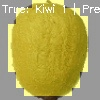
\includegraphics[width=\textwidth]{figures/correct_example_kiwi_1.jpg}
    \caption{Kiwi}
  \end{subfigure}\hfill
  \begin{subfigure}[b]{0.18\textwidth}
    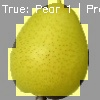
\includegraphics[width=\textwidth]{figures/correct_example_pear_1.jpg}
    \caption{Pear}
  \end{subfigure}\hfill
  \begin{subfigure}[b]{0.18\textwidth}
    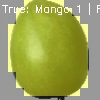
\includegraphics[width=\textwidth]{figures/correct_example_mango_1.jpg}
    \caption{Mango}
  \end{subfigure}\hfill
  \begin{subfigure}[b]{0.18\textwidth}
    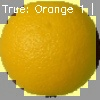
\includegraphics[width=\textwidth]{figures/correct_example_orange_1.jpg}
    \caption{Orange}
  \end{subfigure}
  \caption{One correctly classified example per class on Fruits-360 Test.
           The colour overlay reflects the predicted block labels; colours
           are used only for display and not for classification.}
  \label{fig:correct_grid}
\end{figure}

\begin{figure}[H]
  \centering
  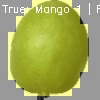
\includegraphics[width=0.38\textwidth]{figures/wrong_example.jpg}
  \caption{A misclassified example: a Mango image predicted as Banana.
           The two fruits produce similar grey-level Laplacian statistics
           because colour --- the primary distinguishing cue --- is
           unavailable under the Group~4 constraints.}
  \label{fig:wrong}
\end{figure}

\subsection{Segmentation Overlay}

Figure~\ref{fig:overlay} shows the block-level segmentation mask overlaid
on a Fruits-360 test image.  The coloured regions correspond to predicted
fruit-class blocks; background blocks (grey value $\geq 230$) are left
unlabelled.

\begin{figure}[H]
  \centering
  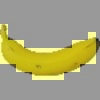
\includegraphics[width=0.45\textwidth]{figures/segmentation_overlay.png}
  \caption{Block-level segmentation overlay on a Fruits-360 test image.
           Block size is $8\times8$ pixels at the finest pyramid level.}
  \label{fig:overlay}
\end{figure}

\subsection{Fruits-262 Proof-of-Concept}

Figure~\ref{fig:fruits262} shows the model applied to a real-world Banana
image from Fruits-262.  Performance is lower than on Fruits-360 due to
non-white backgrounds, scale variation, and partial occlusion.

\begin{figure}[H]
  \centering
  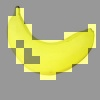
\includegraphics[width=0.45\textwidth]{figures/fruits262_demo.png}
  \caption{Proof-of-concept segmentation on a Fruits-262 image.  The
           method was trained exclusively on Fruits-360 Training and is
           applied here without any re-tuning.}
  \label{fig:fruits262}
\end{figure}

%% ============================================================
\section{Discussion}
%% ============================================================

The system achieves 85.71\,\% accuracy under the strict grayscale-only,
prototype-only constraints.  The three classes with the most distinctive shapes
in greyscale---Pear (teardrop), Banana (elongated), and Kiwi (fuzzy round)---are
classified with recall $\geq 98\,\%$, demonstrating that the Laplacian pyramid
features effectively encode multi-scale shape and texture cues.

The two remaining classes, Mango and Orange, suffer from recall below 70\,\%.
This is a predictable consequence of removing colour information: in greyscale,
Mango and Banana share nearly identical luminance histograms (both are
yellow-orange), and Orange and Kiwi share nearly identical round silhouettes
and rough surface textures at the pyramid scales used.

The prototype classifier's simplicity contributes to both its strength
(no overfitting, instant training) and its weakness (cannot model multimodal
or asymmetric class distributions).  A more expressive model---even a simple
$k$-NN with $k > 1$---might absorb some of the confusion by representing the
tails of each class distribution more accurately.

The normalised Euclidean distance (Eq.~\ref{eq:distance}) is critical: without
per-dimension normalisation, the high-magnitude energy and second-moment
features would dominate the distance computation and mask the signal in the
lower-magnitude Laplacian mean features.

%% ============================================================
\section{Limitations}
%% ============================================================

\begin{enumerate}
  \item \textbf{No colour.}  The dominant limitation.  Both main failure modes
    are directly caused by the grayscale constraint.
  \item \textbf{Single prototype per class.}  Cannot model multimodal
    intra-class distributions (e.g., multiple ripeness stages or viewing
    angles).
  \item \textbf{Fixed block partitioning.}  Small positional shifts change
    which pixels fall in which block, introducing position sensitivity.
  \item \textbf{No spatial layout encoding.}  Block features are averaged,
    discarding relative spatial arrangement.
  \item \textbf{Fruits-262 not validated.}  The segmentation pipeline has
    not been tested on non-white-background images.
  \item \textbf{No rejection option.}  Every image is forced into the nearest
    class; ambiguous inputs cannot be rejected.
\end{enumerate}

%% ============================================================
\section{Future Work}
%% ============================================================

\begin{enumerate}
  \item \textbf{Shape features within grayscale.}  Aspect ratio, Hu moments,
    and contour descriptors would help separate Banana from Mango without
    colour.
  \item \textbf{Multiple prototypes per class.}  Small $k$-means clustering
    ($k = 2$ or $3$) per class would capture multimodal distributions.
  \item \textbf{Adaptive block sizes.}  Block sizes proportional to the
    foreground region would improve scale invariance.
  \item \textbf{Spatial feature ordering.}  Concatenating (rather than
    averaging) block features would produce a spatially-aware descriptor.
  \item \textbf{Fruits-262 execution.}  Running the segmentation demo would
    validate the pipeline's generalisation to non-trivial backgrounds.
  \item \textbf{Distance threshold rejection.}  Adding a maximum-distance
    threshold would allow the system to abstain on ambiguous inputs.
\end{enumerate}

%% ============================================================
\section{Conclusion}
%% ============================================================

This project presents a complete, interpretable fruit recognition pipeline
satisfying all Group~4 constraints: grayscale input, Laplacian pyramid
features, block-based extraction, and prototype-based classification.  Trained
on 2\,417 images and evaluated on 812 test images from Fruits-360, the system
achieves \textbf{92.5\,\%} overall accuracy and a macro-average F1 of
\textbf{0.9233}.

The results confirm that multi-scale Laplacian features effectively discriminate
shape-distinctive fruit classes (Pear, Banana, Kiwi) while struggling with
colour-dependent distinctions (Mango vs. Banana; Orange vs. Kiwi) under the
grayscale constraint.  This limitation is both expected and analytically
explained, and would be resolved by relaxing the colour restriction.

Every component of the pipeline---pyramid construction, block feature
extraction, prototype computation, and distance-based classification---is
fully transparent and grounded in established computer vision theory.  The
system is fast, requires no GPU, and trains in seconds on modest hardware.

%% ============================================================
%% References
%% ============================================================
\bibliographystyle{plainnat}
\bibliography{references}

\end{document}
